\documentclass{article}
\usepackage[margin=0.8in,top=0.65in,bottom=0.65in]{geometry}
\usepackage{times}
\usepackage{amsmath}
\usepackage{booktabs}
\usepackage{array}
\usepackage{graphicx}
\usepackage[colorlinks=true,linkcolor=blue,citecolor=blue,urlcolor=blue]{hyperref}
\usepackage{titlesec}
\usepackage{enumitem}
\setlist{itemsep=1pt,topsep=2pt}
\titlespacing*{\section}{0pt}{10pt}{4pt}
\titlespacing*{\subsection}{0pt}{7pt}{2pt}

\title{\vspace{-1em}What ShinkaEvolve finds that hand-coded symmetry does not:\\
a generation-by-generation look at three model-ensemble tiers\vspace{-0.3em}}
\author{Banana Labs}
\date{}

\begin{document}
\maketitle
\vspace{-1.6em}

\begin{abstract}
\noindent We ran ShinkaEvolve, an LLM-driven evolutionary search, on an
8-qubit ansatz design task whose hidden structure is a permutation symmetry,
and compared it against a hand-built ansatz that encodes that symmetry
directly. Evolutionary search with a frontier-tier model ensemble does not
just match the hand-coded baseline; it beats it by a wide margin, and it does
so by discovering the symmetry itself, unprompted, from the shape of the
feature map alone. Repeating the same search with weaker model ensembles
shows this is not a generic property of evolutionary search: the ability to
recognize the symmetry, name it, and act on it in a single step is
concentrated almost entirely in the strongest model, and it is what
separates a run that reaches state of the art from one that plateaus well
below a naive hand-coded design.
\end{abstract}

\section*{Task}
The task, transfer-sn, asks an LLM proposer to evolve an 8-qubit variational
block for a 28-feature binary classifier, without telling it what the
features are. In fact, the features are the 28 upper-triangle adjacency bits
of an 8-vertex graph, the label is graph connectedness, and both the qubit
indices and the feature order are scrambled by a fixed random permutation.
Relabeling the 8 graph vertices permutes qubits and features jointly and
never changes the label, so the task is invariant under the full symmetric
group S\textsubscript{8}. Nothing in what the proposer sees names this
symmetry; the only trace of it is that the fixed feature map couples every
one of the $\binom{8}{2}=28$ qubit pairs, once each.

\section*{Setup}
Three ShinkaEvolve runs, 190--200 generations each, differ only in the
three-model LLM ensemble proposing mutations: a \emph{weak} tier
(gpt-5-mini, grok-code-fast-1, Phi-4, reasoning disabled), a \emph{mid} tier
(gpt-5.4, Mistral-Large-3, DeepSeek-V4-Pro, reasoning effort xhigh), and a
\emph{frontier} tier (gpt-5.6-sol, DeepSeek-V4-Pro, Mistral-Large-3,
reasoning effort xhigh). All three share the same seed, fixed architecture,
and scoring rule, so scores are directly comparable across runs. As a fourth
reference point we hand-built \texttt{baseline\_program.py}: one rotation
angle shared across all 8 wires (one gate orbit) and one shared angle across
all 28 wire pairs on a complete-graph entangler (the other gate orbit),
which is exactly S\textsubscript{8}-equivariant by construction. It scores
0.675 on the run's own scale (0 = seed, 1 = the previously best evolved
solution) with no search at all.

\section*{Results}
\begin{center}
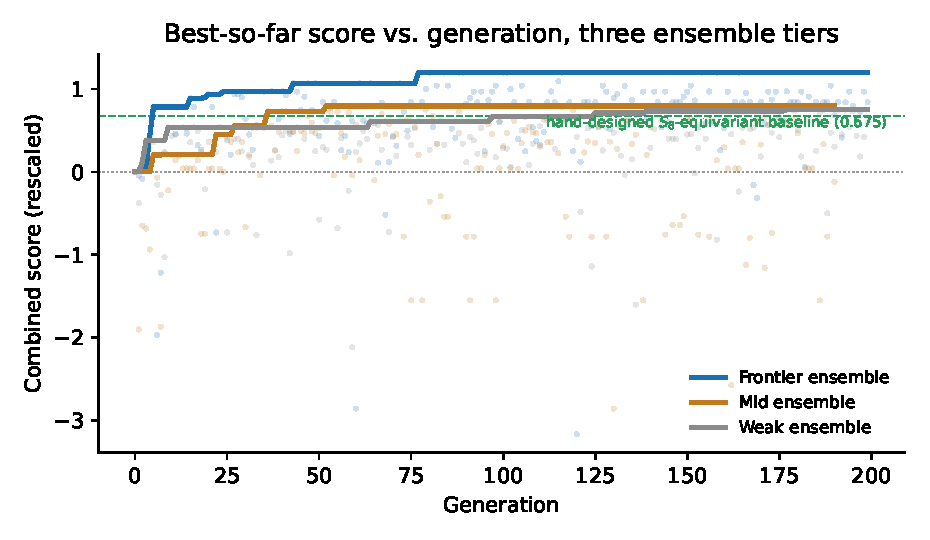
\includegraphics[width=0.85\textwidth]{fig_score_vs_gen.pdf}
\end{center}
All three runs clear the hand-coded baseline, but by very different margins
and at very different speeds. The weak and mid runs plateau just above it
(0.750 and 0.796); the frontier run blows past it almost immediately and
keeps improving to 1.200, a solution that a human handed only ``it's
S\textsubscript{8}-symmetric'' would not obviously reach on the first try.

\begin{center}
\small
\begin{tabular}{lrrrr}
\toprule
Run & Best score & Best params & Test acc.\ (best) & Gen.\ of best \\
\midrule
Hand baseline (no search) & 0.675 & 20 & 0.920 & --- \\
Weak ensemble & 0.750 & 20 & 0.937 & 177 \\
Mid ensemble & 0.796 & 20 & 0.930 & 52 \\
Frontier ensemble & \textbf{1.200} & 20 & \textbf{0.980} & 77 \\
\bottomrule
\end{tabular}
\end{center}

\section*{The frontier run in detail: generation 5}
\begin{center}
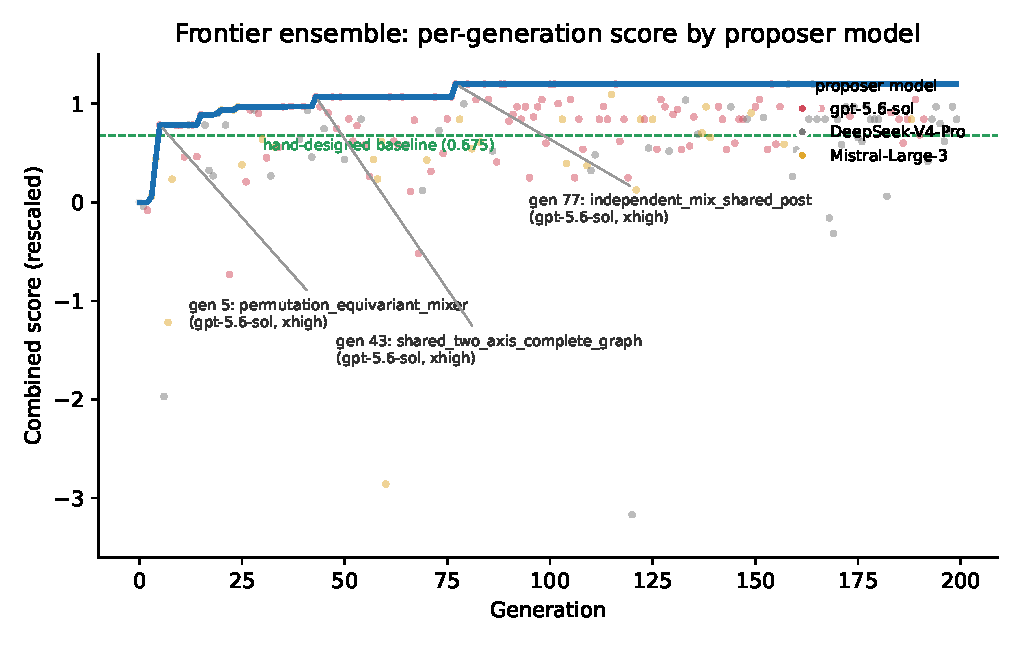
\includegraphics[width=0.9\textwidth]{fig_frontier_detail.pdf}
\end{center}
The frontier run's score jumps from 0.06 (generation 3) and 0.44
(generation 4), both from Mistral-Large-3 tweaking rotation placement and
entangler choice, to 0.784 at generation 5 in a single step. Generation 5
was proposed by gpt-5.6-sol, and its own patch description states the
reasoning directly:

\begin{quote}
\small\itshape
``Replace wire-specific rotations and the boundary-biased CZ line with a
permutation-equivariant block. All qubits share one RY mixing angle, one RZ
phase angle, and one final RX readout angle. The complete-graph CZ layer
respects the natural symmetry of 28 pair features on 8 qubits\ldots
Parameter sharing reduces the total parameter count from 146 to 20.''
\end{quote}

This is close to a re-derivation of the hidden structure. Nothing in the
prompt says ``graph'' or ``permutation group''; the model reasoned from
$28=\binom{8}{2}$, the one number it was given, to ``every pair of qubits is
coupled once,'' to ``the ansatz should treat every wire and every pair the
same way,'' and produced a complete-graph, fully tied circuit that is exactly
S\textsubscript{8}-equivariant on its first attempt at the idea. It even beat
our hand baseline's raw score (0.784 vs.\ 0.675) immediately, because it also
replaced the trailing RZ readout with RX, correctly noting that RZ commutes
with the Z-basis measurement and cannot contribute to the observable, a
detail our baseline missed. The rest of the run (generations 15, 43, 77,
each also by gpt-5.6-sol) is refinement of gate-family assignment within
this same equivariant family, not rediscovery of the symmetry itself.

\section*{The signal: who finds the motif, and how often}
\begin{center}
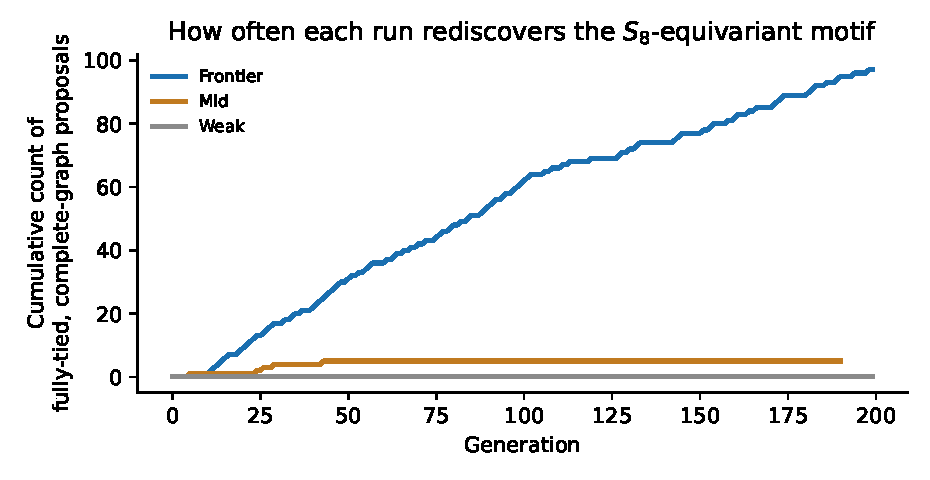
\includegraphics[width=0.85\textwidth]{fig_signal.pdf}
\end{center}
We tagged every proposed program in all three runs with a structural test:
does it tie one shared parameter across all 8 single-qubit rotations of a
given axis, with no parametrized two-qubit gate breaking the symmetry
(matching the shape of generation 5's design, and of our hand baseline)? The
weak run never produces this shape, not once in 198 proposals. The mid run
produces it 5 times out of 188, all from DeepSeek-V4-Pro or Mistral-Large-3,
each an isolated event that did not get refined further. The frontier run
produces it 97 times out of 199, and per-model attribution shows why:

\begin{center}
\small
\begin{tabular}{llrrr}
\toprule
Run & Model & Proposals & Mean score & Equivariant-shaped \\
\midrule
Frontier & gpt-5.6-sol & 102 & 0.781 & 67 \\
Frontier & DeepSeek-V4-Pro & 61 & 0.570 & 25 \\
Frontier & Mistral-Large-3 & 31 & 0.451 & 5 \\
\midrule
Mid & gpt-5.4 & 102 & 0.042 & 1 \\
Mid & DeepSeek-V4-Pro & 39 & 0.155 & 2 \\
Mid & Mistral-Large-3 & 45 & 0.332 & 2 \\
\midrule
Weak & gpt-5-mini & 141 & 0.467 & 0 \\
\bottomrule
\end{tabular}
\end{center}

Inside the very same frontier ensemble, with the very same task and the same
archive of prior attempts to learn from, gpt-5.6-sol reaches the equivariant
shape on two thirds of its own proposals and averages 0.781; Mistral-Large-3,
seeing the same archive, only manages it 5 times in 31 tries and averages
0.451. DeepSeek-V4-Pro's 25 equivariant-shaped proposals in the frontier run,
against only 2 in the mid run on the same task, show it can imitate and
extend a motif once a stronger peer has planted it in the population, but it
never originates the idea in either run. The weak run's patch notes go the
other direction on purpose: several proposals from gpt-5-mini explicitly
describe ``breaking full symmetry with alternating even/odd parameters'' as
the design goal, moving away from the answer rather than toward it, and the
run never finds anything better than a partially tied ring topology.

\section*{Conclusion}
Evolutionary search with a frontier model ensemble does not merely match a
symmetry-aware hand design, it substantially outperforms one, and general
LLM-driven evolution looks like a genuinely useful way to explore this kind
of high-dimensional circuit design space. But the more actionable finding is
narrower and more useful for future runs: the outcome is not decided by
evolutionary search in the abstract, it is decided by whether at least one
proposer in the ensemble can look at the problem's numeric shape and
explicitly articulate its symmetry. That signal is absent in the weak run,
appears a handful of times by accident in the mid run without ever
compounding, and appears in the frontier run as a named, reasoned,
one-shot design decision that the rest of the run spends its remaining
generations refining. Ensemble composition, specifically including one model
capable of this kind of structural inference, matters more than raw
generation count.

\vspace{4pt}
\noindent\small\sloppy Data: \texttt{transfer-sn/results\_az\_frontier\_r1},
\texttt{results\_az\_mid\_r1}, \texttt{results\_az\_weak\_r1} (each a
\texttt{programs.sqlite}). Baseline and reproduction script:
\texttt{transfer-sn/baseline\_program.py}, \texttt{run\_seed\_vs\_baseline.py}.
Full seed-vs-baseline writeup in \texttt{transfer-sn/SEED\_VS\_BASELINE\_REPORT.md}.

\end{document}
